\newcommand{\nsubparagraph}[1]{\subparagraph{\textbf{#1}}}
\newcommand{\AVG}{\mathit{AVG}}

\section{Empirical Evaluation}\label{sec:empiricalEvaluation}
In this section all six identification methods are analyzed in terms of their process to obtain the catalog candidate
set $R$, their catalog set $r$ selection process, and their bijection $h$ production process under varying amounts
of false stars and Gaussian noise.
The main areas of interest here are the accuracy of each step, and the time to produce a result.

\subsection{Experimental Setup}\label{subsec:experimentalSetup}
\begin{subequations}
    \nsubparagraph{Star Catalog:}
    The star catalog used for $K$ is the Hipparcos Input Catalogue~\cite{perryman:hipparcosCatalogue}.
    Entries that do not have a point $\left( \alpha, \delta \right)$ associated with it were not recorded, giving
    117,956 total stars.
    Out of this entire set, only 4,560 are visible from Earth with the naked eye (apparent magnitude $m$ less than 6.0).
    An additional constraint for each catalog $K^2, K^3, \bar{K^3}$ that all stars in each pair or trio be within 20
    degrees of each other was placed to shorten each algorithm's query step running time.
    A field-of-view between 10 to 20 degrees is common for most astronomy based CCD
    cameras~\cite{motari:pyramidIdentification}.
    All sets $K^2, K^3, \bar{K^3}$ construct combinations and permutations using the 4,560 elements and this field
    of view constraint.

    Each entry in $K$ was also been updated from MJD 48319 (March 1991) to MJD 58119 (January 2018).
    The conversion to obtain these updated positions is given below:
    \begin{align}
        \alpha_t &= \alpha_{0} + \mu_\alpha (t_0 - t) \\
        \delta_t &= \delta_{0} + \mu_\delta (t_0 - t)
    \end{align}
    where $\mu_\alpha$ and $\mu_\delta$ represent the proper motion of some star's right ascension and declination in
    radians per year, $\alpha_{0}$ and $\delta_{0}$ represent the right ascension and declination at time
    $t_0$, $t_0$ represents the time the catalog was recorded, and $t$ represents the time we want to update
    our stars to~\cite{nash:3dMotionsAstronomy}.
    To construct the point $[ x \ y \ z ]$ for $K$,~\autoref{eq:sphereToCartesian} was used with
    each new $\left(\alpha_t, \delta_t \right)$, with $r = 1$, and then normalized.
\end{subequations}

\nsubparagraph{Benchmark Data Generation:}
Before a raw image can be used in any of the star identification algorithms presented above, it must go through
three major processes: blob detection, centroid determination, and a 2D $\rightarrow$ 3D transformation process.
If a blob is not wholly detected, the centroid is not determined correctly, or the transformation process
is not precise enough, error will exist as input to the algorithm prior to starting.
Given that our goal is to only characterize each star identification algorithm itself, the solution implemented here
involves generating artificial images in some quasi 3D space.

Prior to generating the benchmark data, three items are specified: a field of view $\psi$, a true attitude
$A^{\nicefrac{\iFrame}{\kFrame}}$, and a 3D vector $\vv{r_f}$ in the catalog frame $\kFrame$ that determines
the center of the image.
The next step is to find all nearby bright stars to the $\vv{r_f}$ in the catalog.
This is denoted as $J$:
\begin{equation}
    J = \set{ j \mid j \in K \land \theta\left( j, \vv{r_f} \right) < \frac{\psi}{2} }
\end{equation}
To get the $I$ set, each star in $J$ is then rotated by the true attitude $A^{\nicefrac{\iFrame}{\kFrame}}$:
\begin{equation}
    I = \set{ A^{\nicefrac{\iFrame}{\kFrame}} \cdot j \mid j \in J }
\end{equation}
The set $I$, the field of view, and the rotated image center $\vv{b_f} = A^{\nicefrac{\iFrame}{\kFrame}} \cdot \vv{r_f}$
are then presented to each star identification algorithm.

The first type of noise exists as variance between the relative positions of stars represented in the catalog and those
represented in the image.
This may come from misidentifying the centroids in the image or out-of-date catalogs.
To introduce Gaussian noise to an image, we spherically linearly interpolate each star toward some random 3D vector on
the unit sphere (\textit{SLERP}) and distribute the magnitude of the movement normally.
To describe our noise independent of this random vector, we divide a normal random variable by the current angular
separation between both stars.
Given a star $b_i \in I$, Gaussian noise is applied to obtain the distributed vector $b'_i$~\cite{kremer:slerp}:
\begin{equation}
    b'_i &= \frac{\sin (1 - K)\Omega}{\sin \Omega}b_i + \frac{\sin \left( K \Omega )\right}{\sin \Omega}b^\star_i
\end{equation}
\begin{subequations}
    where $b^\star_i$ represents some random vector with uniformly distributed elements, $\Omega$ describes the
    angle subtended by the arc, and $K$ describes the magnitude of the interpolation.
    $\rho$ in the equation below represents the standard deviation of noise.
    \begin{align}
            b^\star_i &= \left[ \sim U(-1, 1), \sim U(-1, 1), \sim U(-1, 1) \right] \\
            \Omega &= \arccos \left ( b^{\star}_i \cdot b_i \right) \\
            K &= \left(\sim N\left(0, \rho^2\right)\right) \cdot \left(\theta\left( b^{\star}_i, b_i \right)
            \right)^{-1}
    \end{align}
    The additional constraint that the resulting star exist near the image center is also applied:
    $\theta\left( b'_i, \vv{r_f} \right) < \nicefrac{\psi}{2}$.
    If this is not met, then the process is repeated for this star.
\end{subequations}

The second type of noise exists as falsely identified sources of light, or spikes in the image.
This involves generating $b^\star_i$ in the same manner that was done for the Gaussian noise process, and normalizing
this.
If the constraint that $b^\star_i$ be near the image center is not met, this process is repeated until such a star is
found.
This is repeated for a set number of spikes.

\nsubparagraph{Hardware:}
All trials were performed on an Intel i7-7700 CPU, 3.60GHz with 8 GB RAM\@.
Each algorithm was implemented in C++14, and compiled without optimization (at \texttt{-O0}).
The exact implementation is available at the following link:
\url{https://github.com/glennga/hoku}.

\newpage
\subsection{Catalog Query Step}\label{subsec:catalogQueryStep}
\nsubparagraph{Determining Query $\sigma$:}
In all predicates used to query the catalog, an assumption must be made about the difference between the catalog
measurements and the image measurements.
If this deviation assumption $\sigma$ is too large, false positives will exist in $R$ after querying and may slow
down identification.
On the other hand, $\abs{R} = 0$ if the deviation assumption is too small.
The heuristic used to determine each query $\sigma$ was a grid search, iteratively exhausting every permutation of
deviations in the set below for 30 query steps each:
\begin{equation}
    \sigma_{gd} \in \set{ 10^{-16}, 10^{-15}, \ldots, 10^1 }
\end{equation}
As an example, the Dot Angle method of $\abs{\omega} = 2$ would have $18^2$ distinct parameter sets with 30 runs
attached to each set.
The Angle method of $\abs{\omega} = 1$ would have $18$ distinct parameter sets with 30 runs attached to each set.
The parameter sets with the largest $\sigma$ choices but most number of instances where $\abs{R} = 1$ were selected.

The results of each grid search are displayed below, and were used for the following experiments.
\begin{alignat*}{3}
    \text{Angle}&: \sigma_\theta &&= 10^{-4} &&{}\\
    \text{Pyramid}&: \sigma_\theta &&= 10^{-4} &&{} \\
    \text{Dot Angle}&: \sigma_\theta_ &&= 10^{-2}, \sigma_\phi &&= 10^{-2} \\
    \text{Spherical Triangle}&: \sigma_a &&= 10^{-9}, \sigma_\imath &&= 10^{-9} \\
    \text{Planar Triangle}&: \sigma_a &&= 10^{-9}, \sigma_\imath &&= 10^{-9} \\
    \text{Composite Pyramid}&: \sigma_a &&= 10^{-9}, \sigma_\imath &&= 10^{-9}
\end{alignat*}

\begin{table}
    \centering {
    %\begin{tabular}{m{0.22\columnwidth}|m{0.2\columnwidth}|m{0.2\columnwidth}|m{0.2\columnwidth}} \toprule
%    \textit{Method} & $y'$ & $S$ & $t_{\AVG} \ (\si{ms})$  \\ \hline
%    Angle & \num{2000} & \num{32} & \num{138.00} \\ \hline
%    Dot Angle & \num{2000} & \num{1440} & \num{171.80} \\ \hline
%    Planar \newline Triangle & \num{2000} & \num{1994} & \num{139.05} \\ \hline
%    Composite \newline Pyramid & \num{2000} & \num{1991} & \num{139.46} \\ \hline
%    Spherical \newline Triangle & \num{2000} & \num{1984} & \num{139.60} \\ \hline
%    Pyramid & \num{1980} & \num{1501} & \num{149.69} \\ \bottomrule
%\end{tabular}

\begin{tabular}{m{0.22\columnwidth}|m{0.2\columnwidth}|m{0.2\columnwidth}|m{0.2\columnwidth}}
    \toprule
    \textit{Method} & $P(r_b \in R)$ & $S$ & $t_{\AVG} \ (\si{ms})$  \\ \hline
    Angle & \num{1.0} & \num{32} & \num{138.00} \\ \hline
    Dot Angle & \num{1.0} & \num{1440} & \num{171.80} \\ \hline
    Planar \newline Triangle & \num{1.0} & \num{1994} & \num{139.05} \\ \hline
    Composite \newline Pyramid & \num{1.0} & \num{1991} & \num{139.46} \\ \hline
    Spherical \newline Triangle & \num{1.0} & \num{1984} & \num{139.60} \\ \hline
    Pyramid & \num{0.99} & \num{1501} & \num{149.69} \\ \bottomrule
\end{tabular}
    \caption{
    Depicts all data associated with testing the query step: the frequency of correct catalog sets ($r_b$,
    such that the correct bijection can be formed with $b$) existing in $R$ after querying, the number of trials 
    where the resulting $R$ meets the $\abs{R} = 1$ criterion ($S$),
    and the average query running time ($t_{\AVG}$) given images with no noise.
    There exist 2000 runs for each identification method.
    } \label{tab:queryExperimentResults}
    }
\end{table}

\subsubsection{Which method has the fastest catalog query step?}
In~\autoref{sec:starIdentificationMethods}, we describe each method's running time in terms of the number of catalog
accesses $n$ and the size of the $K^d$ catalog.
The $K^2$ catalog, used by the Angle and Pyramid methods, is of size $m_2 = 353,700$ elements with the apparent
magnitude and field-of-view constraints.
The $K^3$ catalog, used by the Spherical Triangle, Planar Triangle, and Composite Pyramid methods is of size
$m_3 = 12,520,359$ elements.
The $\bar{K^3}$ catalog, used by the Dot Angle method is of size $\bar{m_3} = 37,561,083$ elements.
Given the size of each catalog, we expect that the Angle method will have the fastest query step
(Pyramid method accesses $K^2$ three times in query step) and the Dot Angle will have the slowest query step.

In~\autoref{tab:queryExperimentResults}, the average running time to obtain an $R$ set is displayed for each
identification method given an image for 2000 runs.
The slowest method on average is the Dot Angle method, with its $t_{\AVG} = 30.64 \si{ms}$ longer than the average
$t_{\AVG}$ for all other methods ($141.16 \pm 4.30 \si{ms}$).
Rore time is being spent searching for the appropriate elements.

%# http://www.socscistatistics.com/pvalues/normaldistribution.aspx
%import numpy as np
%m_1, m_2, s_1, s_2, n_1, n_2 = 137.9965, 139.051, 4.201486373891982, 3.3748183654828003, 2000, 2000
%z_plane = (m_2 - m_1) / np.sqrt( ((s_1 * s_1) / n_1) + ((s_2 * s_2) / n_2) )
We note that the two fastest methods appear to be Angle method and the Planar Triangle method, but their $t_\AVG$ only
vary by 1.05ms.
Given the null hypothesis that the difference between the Planar Triangle method's query step running time and the
Angle method's query step running time is not significant, $z = 8.75, p < 0.0001$ is found with a two-tailed two
sample $Z$ test.
The Angle method has the fastest query step due its small catalog size.

\subsubsection{Which method meets the $\abs{R} = 1$ criterion the most often?}
The $\abs{R} = 1$ criterion is required for all identification methods at some point (after pivoting for the triangle
methods), and meeting this criteria as often as possible prevents additional catalog accesses from occurring.

In~\autoref{tab:queryExperimentResults}, the lowest number of instances where the criterion is met $S$ lies with the
Angle method.
Out of 2000 query steps, the Angle method will have had to perform an additional query step at least 1968 more times.
The Pyramid method only has 499 of these additional query instances, which is a factor of 3.94 less.
The most likely reason for this lies with the selection of the $\sigma_\theta$ parameter, and the fact that only one
feature is used to query $K^2$.
If $\sigma_\theta$ was chosen to be smaller, there would have been more instances where the criterion was met- but
this comes at the cost of being less flexible with Gaussian noise.
The methods using $K^3$ and $\bar{K^3}$ have the advantage of being able to create utilize more features of the $b$ set and
distinguish it better, compared to only using $\theta(b, r)$ as the sole feature.

\begin{figure}
    \begin{align*}
        \texttt{SELECT } &r \\
        \texttt{FROM } &K^d \\
        \texttt{WHERE } &g_1(r) < g_1(b) + 3\sigma_{g1} \texttt{ AND } g_1(r) > g_1(b) - 3\sigma_{g1} \texttt{ AND } \\
        &g_2(r) < g_2(b) + 3\sigma_{g2} \texttt{ AND } g_2(r) > g_2(b) - 3\sigma_{g2} \texttt{ AND } \\
        &\vdots \\
        &g_d(r) < g_d(b) + 3\sigma_{gd} \texttt{ AND } g_d(r) > g_d(b) - 3\sigma_{gd}
    \end{align*}
     \caption{
     Depicts a generalized SQL query used for the Angle, Spherical Triangle, Planar Triangle, and Composite Pyramid
     methods.
     Here, $d$ represents the number of stars used in the query, $g$ represents the function used to obtain a feature,
     and $\sigma$ refers to the deviation of noise.
     }\label{fig:sqlQuery}
\end{figure}

%import numpy as np
%p_1, p_2, n_1, n_2 = (1501 / 2000), ((1994 + 1991 + 1984) / 6000), 2000, 6000
%p = (1501 + 1994 + 1991 + 1984) / (2000 + 6000)
%z = (p_2 - p_1) / np.sqrt( p * (1 - p) * ((1/n_1) + (1/n_2)) )
It appears that the all methods using triangular features (Planar Triangle, Composite Pyramid, Spherical Triangle)
meet the criterion the most often (average of $1989.7 \pm 4.2$ runs).
Again, a larger $\sigma_a$ or $\sigma_\imath$ query parameter may lead to a larger $\abs{R}$.
The next method with the most $\abs{R} = 1$ runs that does not use triangular features is the Pyramid method,
which has a factor of 0.75 less runs.
Methods with triangular features are more likely on average to have more instances where the $R$ criterion is met
when compared to methods with angular features.
%Given the null hypothesis that the difference between the number of $\abs{R} = 1$ Pyramid method runs and the
%number of $\abs{R} = 1$ runs for methods with triangular features is not significant, $z = 38.0, p < 0.0001$ is
%obtained with a two proportion $Z$ test.

\subsubsection{How effective is the Pyramid method query?}
In the Angle, Spherical Triangle, Planar Triangle, and Composite Pyramid methods, catalog queries can be
generalized to the query in~\autoref{fig:sqlQuery}.
The Dot Angle method requires the $\theta(r_{c1}, r_{c}) < \theta(r_{c2}, r_c)$ constraint before performing the query
above, but the Pyramid method has the most involved query that involves processing outside of SQL\@.
Three of the queries above must be performed to obtain the $T$ sets, and the common stars must be
found among each $R$ set to create a singular candidate set for trios.

%# http://www.socscistatistics.com/pvalues/normaldistribution.aspx
%import numpy as np
%m_1, m_2, s_1, s_2, n_1, n_2 = 0.99, 1.0, 0.09949874371066202, 0, 2000, 2000
%z = (m_2 - m_1) / np.sqrt( ((s_1 * s_1) / n_1) + ((s_2 * s_2) / n_2) )
There exist several areas where the Pyramid could drop in accuracy in its query.
In~\autoref{tab:queryExperimentResults}, the frequency of the correct $r$ existing in $R$for some $b$ is displayed
for each identification method.
The Pyramid method is shown to have a 0.01\% difference from the 100\% accuracy of each other method.
Given the null hypothesis that this difference is not significant, $z= 4.49, p < 0.0001$ is obtained with a one tailed
two sample $Z$ test.
We find that the Pyramid method's query step is less accurate than other identification methods.
Although small, this error will propagate to the next steps and will result in more catalog accesses and/or a lower
average accuracy.

\subsection{Candidate Selection Step}\label{subsec:candidateSelectionStep}
\begin{figure}
    \centering{
    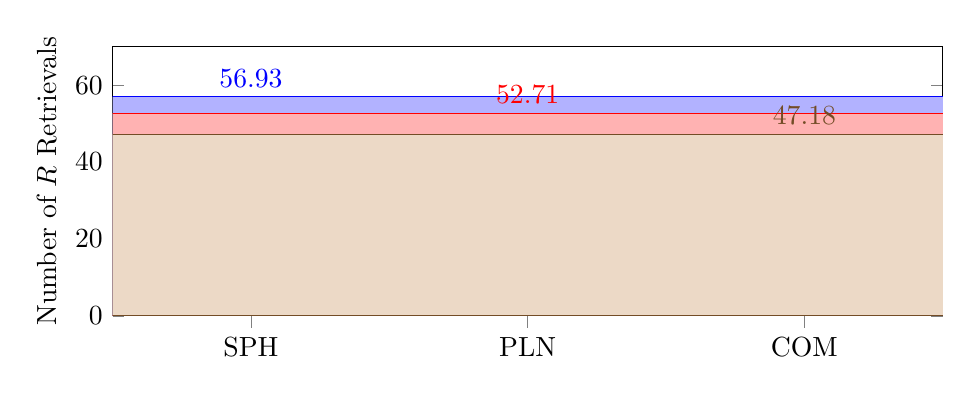
\begin{tikzpicture}
    \begin{axis}[
    ybar,
    width=\linewidth, height=5cm,
    ylabel={Number of $R$ Retrievals}, ylabel near ticks, ymin=0, ymax=70,
    xticklabels={SPH, PLN, COM},
    xtick={1, 2, 3}, xmin=0.5, xmax=3.5, xtick pos=left,
    nodes near coords, nodes near coords align={vertical},
    every axis plot/.append style={
    ybar,
    bar width=40,
    bar shift=0pt,
    fill
    }
    ]
        \addplot coordinates {(1, 56.93)}; % SPH
        \addplot coordinates {(2, 52.71)}; % PLN
        \addplot coordinates {(3, 47.18)};
    \end{axis}
\end{tikzpicture}

%SELECT AVG(QueryCount), IdentificationMethod
%FROM REDUCTION
%WHERE rowid IN (
%    SELECT rowid
%    FROM REDUCTION
%    WHERE (IdentificationMethod LIKE 'Plane' OR IdentificationMethod LIKE 'Sphere')
%    AND ShiftDeviation < 1.0e-3 AND ShiftDeviation > 1.0e-5 AND FalseStars = 0
%    AND QueryCount > 1
%)
%GROUP BY IdentificationMethod

%SELECT AVG(QueryCount)
%FROM REDUCTION
%WHERE rowid IN (
%    SELECT rowid
%    FROM REDUCTION
%    WHERE IdentificationMethod LIKE 'Composite'
%    AND ShiftDeviation < 1.0e-3 AND ShiftDeviation > 1.0e-5 AND FalseStars = 0
%    AND QueryCount > 1
%)
    \caption{
    Depicts the average number of catalog accesses required to obtain a $r$ set for methods with triangular
    features given $\rho = \ang{0.0001}$ of Gaussian noise.
    To characterize the pivoting method itself, we only display instances where $\abs{R} \neq 1$ with the first $b$
    selection.
    The Spherical Triangle method (SPH) has 1952 / 2000 runs matching the criteria before, the Planar Triangle
    method (PLN) has 1946 runs, and the Composite Pyramid (COM) method has 1957 runs.
    }\label{fig:rPivot}
    }
\end{figure}

\subsubsection{How expensive is the pivoting process?}
%import numpy as np
%m_1, m_2, s_1, s_2, n_1, n_2 = 52.71, 47.18, 56.794658219949106, 47.01765577951369, 1946, 1957
%z = (m_2 - m_1) / np.sqrt( ((s_1 * s_1) / n_1) + ((s_2 * s_2) / n_2) )
As seen previously, identification methods with triangular features have the most number of instances where
$\abs{R} = 1$ given an image with no noise.
In~\autoref{fig:rPivot}, the average number of catalog accesses are displayed for these same methods where the first
$b$ selection does not meet the $R$ criterion given an image with Gaussian noise.
We note that the average number of catalog accesses is higher in methods that use the pivoting processes,
as opposed to those that do not.
Given the null hypothesis that the difference between the Planar Triangle method's number of catalog accesses and
the Composite Pyramid method's number of catalog accesses is not significant, $z = 3.3, p < 0.0001$ is
obtained with a two-tailed two sample $Z$ test.
With the data collected here, we find that the pivoting process results in more catalog accesses on average.
This increased number of catalog accesses results in a $6.70\si{ms}$ difference on average between the two.

The pivoting process was only tested with the methods most frequently meeting the $R$ criterion.
An area of interest would be to see the effects of applying this process to methods with angular features (i.e.\ Angle,
Dot Angle, Pyramid).
These methods met the criterion less frequently, and would likely benefit from attempting to reduce the $R$ set before
deciding to choose another $b$ set.

\subsection{Identification Step}\label{subsec:identificationStep}
\begin{figure}
    \centering{
        \begin{tikzpicture}
    \begin{axis}[
    ybar,
    width=\linewidth, height=5cm,
    ylabel={$a(h, b, r)$}, ylabel near ticks, ymin=0, ymax=1.3,
    xtick={1, 2, 3}, xticklabels={$\ang{0}$, $\ang{0.000001}$, $\ang{0.001}$},
    xlabel={$\sigma$ of Noise (degrees)}, xmin=0.5, xmax=3.5, xtick pos=left,
    nodes near coords, every node near coord/.append style={rotate=90, anchor=west},
    legend style={at={(0.5,-0.35)}, anchor=north,legend columns=-1},
    bar width=7
    ]
        \addplot coordinates {(1, 0.999416666666667) (2, 0.999222222222222) (3, 0.354333333333333)};
        \addplot coordinates {(1, 0.956083333333329) (2, 0.954444444444449) (3, 0.203166666666665)};
        \addplot coordinates {(1, 1.0) (2, 1.0) (3, 0.0)};
        \addplot coordinates {(1, 1.0) (2, 0.999833333333333) (3, 0.346333333333333)};
        \legend{PYR, PYR-N, COM, COM-N}
    \end{axis}
\end{tikzpicture}
        \caption{
        Depicts the frequency of correct bijections ($a(h, b, r)$) formed with and without the verification step of
        both the Pyramid and Composite Pyramid methods.
        There exists 2000 runs for each identification method, with a 500 catalog access limit.
        PYR corresponds to the Pyramid method with the verification step, PYR-N corresponds to the Pyramid method
        without the verification step, COM corresponds to the Composite Pyramid method with the verification step,
        and COM-N corresponds to the Composite Pyramid method without the verification step.
        }\label{fig:verify}
    }
\end{figure}

\begin{figure*} % HAD TO MOVE THIS GUY TOO...
    \centering{
    \begin{subfigure}[b]{0.48\linewidth}
        \begin{tikzpicture}
    \begin{axis}[
    ybar,
    width=\linewidth, height=5cm,
    ylabel={$t \ (\si{ms})$}, ylabel near ticks, ymin=10, ymax=100000,
    xtick={1, 2, 3}, xticklabels={$\ang{0}$, $\ang{0.0001}$, $\ang{0.01}$},
    xlabel={$\sigma$ (degrees)}, xmin=0.5, xmax=3.5, xtick pos=left, point meta=rawy,
    nodes near coords, every node near coord/.append style={rotate=90, anchor=west,
    /pgf/number format/.cd,fixed,precision=6},
    legend style={at={(0.5,-0.35)}, anchor=north,legend columns=-1},
    bar width=7, ymode=log, log origin=infty, max space between ticks=20
    ]
        \addplot coordinates {(1, 1197.43) (2, 1349.07) (3, 6509.00)};
        \addplot coordinates {(1, 160.68) (2, 161.80) (3, 872.22)};
        \addplot coordinates {(1, 323.94) (2, 339.23) (3, 392.29)};
        \addplot coordinates {(1, 324.35) (2, 328.85) (3, 352.24)};
        \addplot coordinates {(1, 170.79) (2, 171.53) (3, 364.04)};
        \addplot coordinates {(1, 405.53) (2, 1545.45) (3, 362.30)};
        \legend{ANG, INT, SPH, PLN, PYR, COM}
    \end{axis}
\end{tikzpicture}
    \end{subfigure}
    \begin{subfigure}[b]{0.48\linewidth}
        %if __name__ == '__main__':
%    from numpy import std, average, sqrt, polyfit, log
%    from sqlite3 import connect
%    from os import environ
%
%    conn_1 = connect(environ['HOKU_PROJECT_PATH'] + '/data/lumberjack-all-triad.db')
%    cur = conn_1.cursor()
%
%    # 1,   2,      3,      4,      5,     6,    7,   8
%    # 0.0, 1.0e-6, 1.0e-5, 0.0001, 0.001, 0.01, 0.1, 1.0
%
%    for d in [[1, 2, 3, 4, 5, 6, 7, 8], [0.0, 1.0e-6, 1.0e-5, 0.0001, 0.001, 0.01, 0.1, 1.0]]:
%        t = polyfit(log(d[3:]), [0.9725, 0.386, 0.0035, 0.0, 0.0], 1)
%        print('Angle: {}*ln(x) + {}'.format(t[0], t[1]))
%
%        t = polyfit(log(d[4:]), [0.9885, 0.7055, 0.033, 0.00383333333333333], 1)
%        print('Dot: {}*ln(x) + {}'.format(t[0], t[1]))
%
%        t = polyfit(log(d[2:]), [0.9715, 0.8135, 0.259, 0.0253333333333333, 0.0095, 0.00716666666666667], 1)
%        print('Sphere: {}*ln(x) + {}'.format(t[0], t[1]))
%
%        t = polyfit(log(d[2:]), [0.9865, 0.8615, 0.332166666666667, 0.0245, 0.0095, 0.00483333333333333], 1)
%        print('Plane: {}*ln(x) + {}'.format(t[0], t[1]))
%
%        t = polyfit(log(d[3:]), [0.999333333333334, 0.354333333333333, 0.0, 0.0, 0.0], 1)
%        print('Pyramid: {}*ln(x) + {}'.format(t[0], t[1]))
%
%        t = polyfit(log(d[1:]), [1.0, 0.65, 0.0035, 0.0, 0.0, 0.0, 0.0], 1)
%        print('Composite: {}*ln(x) + {}'.format(t[0], t[1])), print()

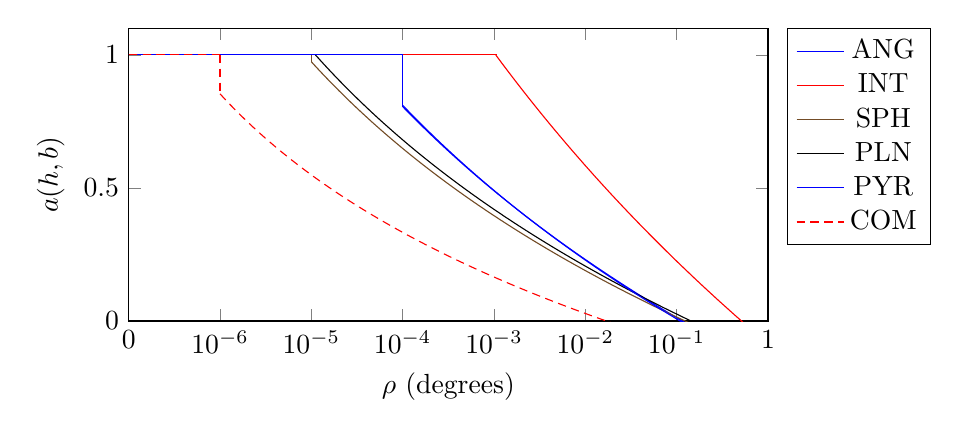
\begin{tikzpicture}
    \begin{axis}[
    width=0.8\linewidth, height=5.3cm,
    ylabel={$a(h, b)$}, ymin=0, ymax=1.1,
    xlabel={$\rho$ (degrees)}, xmin=1, xmax=8,
    xtick={1, 2, 3, 4, 5, 6, 7, 8},
    xticklabels={$0$, $10^{-6}$, $10^{-5}$, $10^{-4}$, $10^{-3}$, $10^{-2}$, $10^{-1}$, $1$},
    samples=100, no markers, legend pos=outer north east, enlargelimits=false
    ]
        \addplot +[domain=1:4, forget plot]{1};
        \addplot +[forget plot] coordinates {(4, 1) (4, 0.8055384229041530)};
        \addplot +[domain=4:8]{-1.416887591459587*ln(x) + 2.7697617012853217};
        \addlegendentry{ANG}

        \addplot +[domain=1:5.03, forget plot]{1};
%        \addplot +[forget plot] coordinates {(5, 1) (5, 1)};
        \addplot +[domain=5.02:8]{-2.3292306442173216*ln(x) + 4.757244753386215};
        \addlegendentry{INT}

        \addplot +[domain=1:3, forget plot]{1};
        \addplot +[forget plot] coordinates {(3, 1) (3, 0.9738787471803161)};
        \addplot +[domain=3:8]{-1.1317828984553227*ln(x) + 2.217269347527745};
        \addlegendentry{SPH}

        \addplot +[domain=1:3, forget plot]{1};
%        \addplot +[forget plot] coordinates {(3, 1) (3, )};
        \addplot +[domain=3.04:8]{-1.1696544292494204*ln(x) + 2.301996347627258};
        \addlegendentry{PLN}

        \addplot +[domain=1:4, forget plot]{1};
        \addplot +[forget plot] coordinates {(4, 1) (4, 0.8105837347641904)};
        \addplot +[domain=4:8]{-1.4347255837709008*ln(x) + 2.7995357213002334};
        \addlegendentry{PYR}

        \addplot +[domain=1:2, forget plot]{1};
        \addplot +[forget plot] coordinates {(2, 1) (2, 0.8533960244900531)};
        \addplot +[domain=2:8]{-0.7510156659772902*ln(x) + 1.3739604159185614};
        \addlegendentry{COM}
    \end{axis}
\end{tikzpicture}
    \end{subfigure}
    \caption{
    Both plots represent some statistic about the resulting bijection $h$ produced by each identification method
    given some image with varying Gaussian noise.
    There exist 2000 runs for each identification method, with a 500 catalog access limit.
    The left plot depicts the average time to obtain $h$, and the right plot depicts the trend line
    $a(h, b, r) = A \cdot \mathit{ln}\left( \rho \right) + B$.
    }\label{fig:gaussianNoise}
    }
\end{figure*}

\subsubsection{How effective are additional verification steps?}
%if __name__ == '__main__':
%from numpy import std, average, sqrt
%from sqlite3 import connect
%from os import environ
%
%conn_1 = connect(environ['HOKU_PROJECT_PATH'] + '/data/lumberjack-all-triad.db')
%conn_2 = connect(environ['HOKU_PROJECT_PATH'] + '/data/lumberjack-pyramid-noverify.db')
%
%name = 'Pyramid'
%
%sample_1 = list(map(lambda b: b.execute("""
%SELECT PercentageCorrect
%FROM IDENTIFICATION
%WHERE ShiftDeviation < 1.0e-7 AND FalseStars = 0
%AND IdentificationMethod LIKE '{}'
%""".format(name)).fetchall(), [conn_1, conn_2]))
%
%sample_2 = list(map(lambda b: b.execute("""
%SELECT PercentageCorrect
%FROM IDENTIFICATION
%WHERE ShiftDeviation < 1.0e-5 AND FalseStars = 0
%AND IdentificationMethod LIKE '{}'
%""".format(name)).fetchall(), [conn_1, conn_2]))
%
%sample_3 = list(map(lambda b: b.execute("""
%SELECT PercentageCorrect
%FROM IDENTIFICATION
%WHERE ShiftDeviation < 1.0e-2 AND ShiftDeviation > 1.0e-4 AND FalseStars = 0
%AND IdentificationMethod LIKE '{}'
%""".format(name)).fetchall(), [conn_1, conn_2]))
%
%flatten = lambda a: [b[0] for b in a]
%for i, sample in enumerate([sample_1, sample_2, sample_3]):
%n_1, n_2 = 2000, 2000
%m_1, m_2 = average(flatten(sample[0])), average(flatten(sample[1]))
%s_1, s_2 = std(flatten(sample[0])), std(flatten(sample[1]))
%print('Z Score of {}: {}'.format(i, (m_2 - m_1) / sqrt( ((s_1 * s_1) / n_1) + ((s_2 * s_2) / n_2) )))

%import numpy as np
%print(np.average( [6.97725 - 3.00525, 6.9615 - 3.005, 398.0655 -  ))
In~\autoref{fig:verify}, the accuracy of the bijection produced by the Pyramid and Composite Pyramid methods are
displayed with and without the verification step for varying levels of Gaussian noise.
Without noise, the Pyramid method without its verification step is 4.33\% less accurate than the Pyramid method with
verification on average.
This behavior is consistently seen for Gaussian noise of $\rho=\ang{0.000001}$ \& $\rho=\ang{0.001}$, and
can be attributed to the more frequent rejection of incorrect bijections with $R$ sets that have met the criterion.
In the $\rho=\ang{0.001}$ case, there exists a difference of 389.95 accesses between both variations of the Pyramid
and a 15\% bijection accuracy difference in favor of the method with the verification step.
Given the null hypotheses that the difference between both variations of the Pyramid method are different for each level
of noise, $z_0 = 15.87, z_{0.000001} = 16.04, z_{0.001} = 12.14$ (all $p < 0.0001$) is obtained with two-tailed two
sample $Z$ tests.
The verification step increases the accuracy of the Pyramid method.

The response to Gaussian noise for the Composite Pyramid begins at $\rho=\ang{0.001}$, with a 34.6\% difference
between the two variants in favor of the method without the verification step.
Unlike the verification step in the Pyramid method, this filter appears to be too aggressive for the Composite Pyramid
method.
The variant without the verification step has an average of 193.93 catalog accesses at $\rho=\ang{0.001}$.
The Pyramid variant without the verification step only had an average of 8.114 catalog accesses, suggesting that the
$\abs{R} = 1$ criterion and the \Call{DMT}{} process are sufficient enough for rejecting incorrect $r$ sets and
bijections for the Composite Pyramid method.

\subsection{End to End}\label{subsec:endToEndEvaluation}
\subsubsection{Which method is the fastest given no noise?}
In~\autoref{fig:gaussianNoise}, the left plot depicts the end to end running time of each identification method given
varying degrees of Gaussian noise.
In the no noise case, the Angle method is the slowest identification method on average.
The next slowest method is the Composite Pyramid method, a factor of 2.95 times faster than the Angle method.
Recall that the Angle method had the fastest query step, but the largest $\abs{R}$.
On average, it takes 69.85 catalog accesses to obtain a bijection and 68.10 catalog accesses to obtain $r$.
This suggests that the Angle method's long running time stems from the $\abs{R} = 1$ criterion and not the \Call{DMT}{}
process.

%import numpy as np
%m_1, m_2, s_1, s_2, n_1, n_2 = 160.675, 170.7905, 0.53808, 0.52922, 2000, 2000
%z = (m_2 - m_1) / np.sqrt( ((s_1 * s_1) / n_1) + ((s_2 * s_2) / n_2) )
The fastest method in the noise case appears to be the Dot Angle method, with the second fastest method running
10.11\si{ms} slower.
There exists 0 / 2000 runs where the Dot Angle method runs above the Pyramid method's average running time
($170.79\si{ms}$) and the Dot Angle method has the fastest recorded identification run of 135ms.
The Dot Angle method is the fastest identification method given no noise.

\subsubsection{Which method is the fastest given varying levels of Gaussian noise?}
As Gaussian noise is increased from $\rho=\ang{0}$ to $\rho=\ang{0.01}$, the Angle method experiences the largest
response of $5311.57$ additional $\si{ms}$.
The next slowest method in the noise of $\rho=\ang{0.01}$ case is the Dot Angle method, a factor of 7.46 times faster
than the Angle method.
On average, the Angle method takes 399.66 catalog accesses to obtain a bijection and only 36.72 catalog accesses
to obtain $r$ here.
In the no noise case, this method's long running time can attributed to the aggressive $R$ criterion.
Given Gaussian noise, the \Call{DMT}{} process plays a larger role with the Angle method and returns to $b$
decision process more often.

The Composite Pyramid method shows an interesting runtime response to this type of noise, running $1139.92\si{ms}$
longer given $\ang{0.0001}$ of noise from no noise but $1183.15\si{ms}$ shorter from $\ang{0.0001}$ of noise to
$\ang{0.01}$.
The Pyramid method is observed to have this same running time response against noise at $\rho=\ang{0.001}$
(not depicted).
The most probable explanation lies in how far each run travels from the $b$ decision step.
At $\rho=\ang{0.0001}$, the Composite Pyramid has gone through the $\abs{R} = 1$ criterion and is likely choosing
another $b$ set after the verification step.
At $\rho=\ang{0.01}$, the Composite Pyramid is not passing the same criterion and does not waste as many catalog
accesses because the verification step is not being performed.

%if __name__ == '__main__':
%from numpy import std, average, sqrt
%from sqlite3 import connect
%from os import environ
%
%conn_1 = connect(environ['HOKU_PROJECT_PATH'] + '/data/lumberjack-all-triad.db')
%conn_2 = connect(environ['HOKU_PROJECT_PATH'] + '/data/lumberjack-pyramid-noverify.db')
%
%sample_1 = conn_1.execute("""
%SELECT TimeToResult
%FROM IDENTIFICATION
%WHERE ShiftDeviation > 1.0e-7 AND FalseStars = 0
%AND IdentificationMethod LIKE 'Plane'
%""").fetchall()
%
%sample_2 = conn_1.execute("""
%SELECT TimeToResult
%FROM IDENTIFICATION
%WHERE ShiftDeviation > 1.0e-7 AND FalseStars = 0
%AND IdentificationMethod LIKE 'Pyramid'
%""").fetchall()
%
%flatten = lambda a: [b[0] for b in a]
%n_1, n_2 = 12000, 12000
%m_1, m_2 = average(flatten(sample_1)), average(flatten(sample_2))
%s_1, s_2 = std(flatten(sample_1)), std(flatten(sample_2))
%print('Z Score of: {}'.format((m_2 - m_1) / sqrt( ((s_1 * s_1) / n_1) + ((s_2 * s_2) / n_2) )))
The fastest method on average given images with the set of Gaussian noise below is the Pyramid method at
$288.44\si{ms}$ (of 12000 runs).
\begin{equation}\label{eq:sigmasTested}
    \rho \in \set{10^{-1}, 10^{-2}, \ldots, 10^{-6}}
\end{equation}
The second fastest method given the same noise set is the Planar Triangle method at $341.16\si{ms}$.
Given the null hypothesis that the difference between both averages is not significant, $z = 24.32, p < 0.0001$ is
found with a two sample $Z$ test.
With the data collected here, the Pyramid method is the fastest method given varying amounts of Gaussian noise.

\subsubsection{Which method has the slowest growing $h$ accuracy response to increasing noise?}
The selection of the query $\sigma$ parameters play a significant role in accuracy of each method given images with
Gaussian noise.
For methods that query the catalog using on the $\theta$ feature (Angle, Dot Angle, Pyramid), the $\sigma$ parameter
serves as a rough upper bound for the amount of Gaussian noise tolerated.
%In~\autoref{fig:gaussianNoise}, the plot on the right depicts the accuracy of resulting bijection of each method for
%varying levels of Gaussian noise.
When the level of noise is equal to the Angle and Pyramid $\sigma_\theta$ parameter ($\ang{0.0001}$),
both methods have an average $h$ accuracy of $98.59 \pm 1.34\%$.
When Gaussian noise is increased to $\ang{0.001}$, both methods drop to $47.02 \pm 1.58\%$.

For methods with features that are not angular (Spherical Triangle, Planar Triangle, Composite Pyramid),
characterizing the effect of Gaussian noise becomes more difficult.
These methods have the query parameters $\sigma_a = 10^{-9}$ and $\sigma_\imath = 10^{-9}$, and first show an
accuracy response to noise at $\ang{0.00001}$.
%The Dot Angle method has the largest query $\sigma$ parameters, and only experiences a response to noise at
%$\ang{0.01}$.
%Given the current set of query $\sigma$, the Dot Angle is the most accurate method on average.

Ranking each method based their $h$ accuracy here is not too insightful, so instead we analyze the rate of change
involved with varying levels of noise.
The right plot in~\autoref{fig:gaussianNoise} depicts the trend line for all methods where $h$ accuracy is displayed
against the amount of Gaussian noise.
Each line was fit to the equation below using least squares:
\begin{equation}
    a(f, b, r) =
    \begin{cases}
        0 & \rho < 0 \\
        1 & 0 \leq \rho < \rho_c \\
        A \cdot \mathit{ln}(\rho) + B & \rho \geq \rho_c
    \end{cases}
\end{equation}
where $A$ and $B$ are the parameters found with the regression, $a(f, b, r)$ is the accuracy of the bijection, and
$\rho_c$ is the point where $a(f, b, r)$ is observed to dip below 95\%.
The acceleration of the accuracy varies across methods through the value of $A$:
\begin{equation}
    \frac{d^{2}a(f, b, r)}{d\rho^2} = \frac{-A}{\rho^2}
\end{equation}
A larger $A$ suggests that a change in query $\sigma$ or Gaussian noise will not affect the accuracy of the method
as much as a method with a larger $A$.
The method with the largest acceleration toward $0\%$ $h$ accuracy is the Dot Angle method ($A = -0.15749$) .
The Spherical Triangle method has the slowest growing $h$ accuracy response to increasing noise ($A = -0.09266$).

\begin{figure*}
    \centering{
    \begin{subfigure}[b]{0.48\linewidth}
        \begin{tikzpicture}
    \begin{axis}[
    ybar,
    width=\linewidth, height=5cm,
    ylabel={$t \ (\si{ms})$}, ylabel near ticks, ymin=10, ymax=100000,
    xtick={1, 2, 3}, xticklabels={0, 6, 12},
    xlabel={$\omega$}, xmin=0.5, xmax=3.5, xtick pos=left, point meta=rawy,
    nodes near coords, every node near coord/.append style={rotate=90, anchor=west,
    /pgf/number format/.cd,fixed,precision=2},
    legend style={at={(0.5,-0.35)}, anchor=north,legend columns=-1},
    bar width=7, ymode=log, log origin=infty, max space between ticks=20
    ]
        \addplot coordinates {(1, 1197.43) (2, 1737.94) (3, 2431.58)};
        \addplot coordinates {(1, 160.68) (2, 209.36) (3, 280.54)};
        \addplot coordinates {(1, 323.94) (2, 355.54) (3, 386.20)};
        \addplot coordinates {(1, 324.35) (2, 350.60) (3, 390.41)};
        \addplot coordinates {(1, 170.79) (2, 183.71) (3, 195.53)};
        \addplot coordinates {(1, 405.53) (2, 685.07) (3, 972.04)};
        \legend{ANG, DOT, SPH, PLN, PYR, COM}
    \end{axis}
\end{tikzpicture}
    \end{subfigure}
    \begin{subfigure}[b]{0.48\linewidth}
        \begin{tikzpicture}
    \begin{axis}[
    ybar,
    width=\linewidth, height=5cm,
    ylabel={Accuracy of Map, \texttt{ACC}}, ylabel near ticks, ymin=0, ymax=1.4,
    xtick={1, 2, 3}, xticklabels={0, 6, 12},
    xlabel={$\omega$}, xmin=0.5, xmax=3.5, xtick pos=left,
    nodes near coords, every node near coord/.append style={rotate=90, anchor=west,
    /pgf/number format/.cd,fixed,precision=4},
    legend style={at={(0.5,-0.35)}, anchor=north,legend columns=-1},
    bar width=7
    ]
        \addplot coordinates {(1, 0.977) (2, 0.979) (3, 0.960)};
        \addplot coordinates {(1, 1.0) (2, 0.982) (3, 0.965)};
        \addplot coordinates {(1, 1.0) (2, 0.840) (3, 0.696)};
        \addplot coordinates {(1, 1.0) (2, 0.845) (3, 0.703)};
        \addplot coordinates {(1, 0.999) (2, 0.999) (3, 0.995)};
        \addplot coordinates {(1, 1.0) (2, 0.994) (3, 0.973)};
        \legend{ANG, INT, SPH, PLN, PYR, COM}
    \end{axis}
\end{tikzpicture}
    \end{subfigure}
    \caption{
    Both plots represent some statistic about the resulting bijection $h$ produced by each identification method
    given some image with varying amounts of spikes $\omega$.
    There exist 2000 runs for each identification method, with a 500 catalog access limit.
    The left plot depicts the average time to obtain $h$, and the right plot depicts the average accuracy of $h$.
    }\label{fig:falseNoise}
    }
\end{figure*}

\subsubsection{Which method is the fastest given varying \\ amounts of false stars?}
In~\autoref{fig:falseNoise}, the plot on the left depicts the end to end running time of each method given varying
amounts of spikes.
As the number of spikes increases from 0 to 12, the Angle method again experiences the largest response of
$1234.15\si{ms}$.
The next slowest method is the Composite Pyramid method, a factor of 2.50 times faster than the Angle method.
The difference between the 1st and 2nd slowest methods is 2.98 times less than the Gaussian noise case.
On average, it takes 114.23 catalog accesses to obtain $h$ and only 54.85 accesses to obtain $r$.
Relative to the Gaussian noise comparison, \Call{DMT}{} and $\abs{R} = 1$ criterion play a more equal role in
the decision to choose a new $b$ set.

%if __name__ == '__main__':
%from numpy import std, average, sqrt
%from sqlite3 import connect
%from os import environ
%
%conn_1 = connect(environ['HOKU_PROJECT_PATH'] + '/data/lumberjack-all-triad.db')
%conn_2 = connect(environ['HOKU_PROJECT_PATH'] + '/data/lumberjack-pyramid-noverify.db')
%
%sample_1 = conn_1.execute("""
%SELECT TimeToResult
%FROM IDENTIFICATION
%WHERE FalseStars > 0
%AND IdentificationMethod LIKE 'Pyramid'
%""").fetchall()
%
%sample_2 = conn_1.execute("""
%SELECT TimeToResult
%FROM IDENTIFICATION
%WHERE FalseStars > 0
%AND IdentificationMethod LIKE 'Dot'
%""").fetchall()
%
%flatten = lambda a: [b[0] for b in a]
%n_1, n_2 = 8000, 8000
%m_1, m_2 = average(flatten(sample_1)), average(flatten(sample_2))
%s_1, s_2 = std(flatten(sample_1)), std(flatten(sample_2))
%print('Z Score of: {}'.format((m_2 - m_1) / sqrt( ((s_1 * s_1) / n_1) + ((s_2 * s_2) / n_2) )))
The fastest method on average given images with the set of spikes below is the Pyramid method at $186.22\si{ms}$
(of 8000 runs).
\begin{equation}\label{eq:numberOfSpikes}
    \omega \in \set{ 3, 6, 9, 12 }
\end{equation}
The second fastest method given the same noise set is the Dot Angle method at $228.37\si{ms}$.
Given the null hypothesis that the difference between both averages is not significant, $z = 28.47, p < 0.0001$ is
found with a two sample $Z$ test.
The Pyramid method is the fastest method given varying amounts of spikes.
The process for choosing distinct image star sets is shown to be effective in finding a bijection that meets the Pyramid
criteria the fastest.

%if __name__ == '__main__':
%from numpy import std, average, sqrt, polyfit, log
%from sqlite3 import connect
%from os import environ
%
%conn_1 = connect(environ['HOKU_PROJECT_PATH'] + '/data/lumberjack-all-triad.db')
%cur = conn_1.cursor()
%
%for name in ['Angle', 'Dot', 'Sphere', 'Plane', 'Pyramid', 'Composite']:
%sample_1 = list(map(lambda a: a[0], cur.execute("""
%SELECT AVG(TimeToResult)
%FROM IDENTIFICATION
%WHERE FalseStars > 0
%AND IdentificationMethod LIKE ?
%GROUP BY FalseStars
%ORDER BY FalseStars
%""", (name, )).fetchall()))
%
%t = polyfit([3, 6, 9, 12], sample_1, 1)
%print('{name}: {t_0}*x + {t_1}'.format(name=name, t_0=round(t[0], 5), t_1=round(t[1], 5)))
Each method exhibits an increase to runtime as additional spikes are added.
To characterize how each method's runtime grows with increasing false stars, each method's runtime was fit to a linear
equation using least squares:
\begin{equation}
    t = A\cdot\omega + B
\end{equation}
where $A$ and $B$ are the parameters found with the regression and $t$ is the end to end running time of the method.
A smaller $\abs{A}$ suggests that the number of spikes will affect the end to end runtime than that of a method with a
larger $\abs{A}$.
The method with the largest $\abs{A}$ is the Angle method with $A = -414.559$.
The method with this smallest $\abs{A}$ term is the Pyramid method with $A = -6.766$.
The Pyramid method is the fastest given varying amounts of false stars, having a runtime that is also the least
responsive to increasing spikes.

\subsubsection{Which method is the most accurate given varying amounts of false stars?}
%if __name__ == '__main__':
%from numpy import std, average, sqrt
%from sqlite3 import connect
%from os import environ
%
%conn_1 = connect(environ['HOKU_PROJECT_PATH'] + '/data/lumberjack-all-triad.db')
%conn_2 = connect(environ['HOKU_PROJECT_PATH'] + '/data/lumberjack-pyramid-noverify.db')
%
%sample_1 = conn_1.execute("""
%SELECT PercentageCorrect
%FROM IDENTIFICATION
%WHERE FalseStars = 12
%AND (IdentificationMethod LIKE 'Plane' OR IdentificationMethod LIKE 'Sphere')
%""").fetchall()
%
%sample_2 = conn_1.execute("""
%SELECT PercentageCorrect
%FROM REDUCTION
%WHERE FalseStars = 12
%AND (IdentificationMethod LIKE 'Plane' OR IdentificationMethod LIKE 'Sphere')
%""").fetchall()
%
%flatten = lambda a: [b[0] for b in a]
%n_1, n_2 = 2000, 2000
%m_1, m_2 = average(flatten(sample_1)), average(flatten(sample_2))
%s_1, s_2 = std(flatten(sample_1)), std(flatten(sample_2))
%print('Z Score of: {}'.format((m_2 - m_1) / sqrt( ((s_1 * s_1) / n_1) + ((s_2 * s_2) / n_2) )))
In~\autoref{fig:falseNoise}, the plot on the right depicts the average accuracy of each bijection given varying amounts
of spikes.
As the number of false stars is increased from $\omega = 0$ to $\omega = 12$, the methods that experience the largest
$h$ accuracy response are the Spherical Triangle method ($30.42\%$ average decrease) and the Planar Triangle method
($29.68\%$ average decrease).
The average accuracy of the $r$ selection is a few percent less than the average accuracy of $h$ here
($0.53 \pm 1.78\%$ for both methods).
Given the null hypothesis that the difference between the accuracy of the $h$ bijection and the accuracy of the $r$
selection is not significant, $z = 0.37, p = 0.71$ was found with a two-tailed two sample $Z$ test.
There does not exist enough data to reject this hypothesis with $\alpha = 0.01$.
This suggests that the \Call{DMT}{} process is neither helpful or detrimental to the end to end accuracy of these
methods.

Ruling out the \Call{DMT}{} process, the most likely source of error for the triangle methods is their decision of
different $b$ sets.
If a false star exists as $b_1$ in $b$, the triangle methods will have to iterate through $n^2$ combinations and $n - 3$
pivots at most to choose another star that is not the spike.
The Angle method only has to wait $n$ additional combinations at most if a false star exists in $b$.
The Dot Angle method is able to get around the spike persistence problem by choosing $b$ sets based on their $\theta$
proximity to the central star $b_c$.
The Pyramid and Composite Pyramid methods have their $b$ decision process designed for this situation, increasing the
average turnover of all stars in the $b$ set.

The Pyramid method has the most accurate $h$ on average given images with $\omega$ in~\autoref{eq:numberOfSpikes}
at $99.84 \pm 3.53\%$.
The second most accurate method is the Composite Pyramid method at $99.19 \pm 8.95\%$.
Given the null hypothesis that the difference between the $h$ accuracies of both methods is not significant,
$z = 3.02, p = 0.003$ with a two-tailed two sample $Z$ test.
At $\alpha = 0.01$, our hypothesis does not hold true.
The Pyramid method is the most accurate under varying amounts of spikes.
